\chapter{Memory Model-Aware Program Analysis}
\label{ch:wmm}

In general, analysis of concurrent programs with respect to axiomatic memory models is performed in several stages. Firstly, the control-flow and data-flow of a program is encoded as the set of possible \textit{candidate executions}. %possible communications between threads of the program.
Obtained model of the program is called an anarchic semantics, which is a truly parallel semantics with no global time that describes all possible computations with all possible communications~\cite{alglave2016syntax}. Thereafter, the anarchic semantics is constrained by the \textit{weak memory model} specification which is a set of axiomatic constraints for filtering out executions inconsistent in particular architecture.


\section{The event-based program representation}
\label{ch:wmm:event}

%"The semantics of a program is a set of executions" https://johnwickerson.github.io/papers/memalloy.pdf

The classical approach to model concurrent programs is to use the \textit{global time}, a single order of interleavings among all events happened in different threads. However these models are easy to understand, it may be impossible to process \textit{all} possible states, number of which is exponentially large. However, there exist some equivalence classes such that the result of execution different interleavings from single equivalence class is the same (for instance, computations performed by a processor locally do not affect the global state).
%One way to do this is to use a non-deterministic computation-centric model~\cite{fri97}, such as ...%The idea in this class of models is based on the fact that the behaviour of a concurrent system is defined only by the interleavings of shared-memory operations, while being independent from the order of local computation events.
One such model is the \textit{event-based} representation of a program, which models a program as a directed graph (the \textit{event-flow graph}). The vertices of such a graph represent \textit{events} (simple low-level instructions; see Section~\ref{ch:wmm:model:events}), and edges represent \textit{relations} over the events (see Section~\ref{ch:wmm:model:relations}). Thus, a candidate execution constitutes the set of guesses which event (from the set of possible next events) is to be executed. 


\subsection{Events}
\label{ch:wmm:model:events}

% TODO: check this subseciton

A \textit{memory event} $e_m \in \mathbb{E}$ represents the fact of access to the memory. Since memory is the crucial low-level resource shared by multiple processes, most relations are defined over memory events. 
The processes can access a shared memory location (denoted by~$l_i$, for \textit{location}), or a local one (denoted by~$r_i$, for \textit{register}). A memory event can access at most one shared memory location, high-level instructions that address more than one shared variable must be transformed into a sequence of events. A memory event is specified by its direction with respect to the shared variable, its location~$\mathtt{loc}(e_m)$, its processor label~$\mathtt{proc}(e_m)$, and a unique event label~$\mathtt{id}(e_m)$~\cite{alglave2010shared}.
%\texttt{load} for read the value of a shared-memory location, or \texttt{store} for write, or neither of them if both locations are local

The set of memory events $\mathbb{M}$ is divided into write events $\mathbb{W}$ (that write values to shared-memory locations) and read events $\mathbb{R}$ (that read values stored in shared-memory locations).
We add a restriction that each memory event uses at most one shared location, so that the write instruction $i = write(l_1, l_2)$, that encodes the write from the shared location $l_2$ to the shared location $l_1$, is represented as two consequent events $e_1~=~\mathtt{load}(r_1~\leftarrow~l_2); \ e_2~=~\mathtt{store}(l_1~\leftarrow~r_1)$.
Also, it is important to separate the set of initial write events $\mathbb{IW}~\subset~\mathbb{W}$ that perform initialisation of program variables.

A \textit{computation event} $e_c \in \mathbb{C} \subseteq \mathbb{E}$, represents a low-level assembly computation operation performed solely on local-memory arguments. An example of computation event may be the event $e_c = r_1 \leftarrow add(r_2, 1)$ that writes the sum of values stored in register $r_2$ and constant $1$ (which is modelled as a register as well) to the register $r_1$. 
For modelling branching statements, we distinguish the set $\mathbb{C_{p}} \subseteq \mathbb{C}$ of \textit{predicative} computation events (also called as \textit{branching events}), that are evaluated as a boolean value.

The synchronisation instructions (fences) cause the \textit{barrier events}, that do not perform any computation or memory value transfer, instead, they add new relations to the program model that restrict the set of allowed behaviours. Semantically, a fence may serve as a synchronisation barrier, or as a flush of local memory caches, etc.


\subsection{Relations}
\label{ch:wmm:model:relations}

%In this section, we describe basic relations used in memory model-aware program analysis.

The relation~$\xrightarrow{r}\,:~\mathbb{E}~\times~\mathbb{E}$ is a binary function over events (set of pairs of events). There are two kinds of relations between events: \textit{basic relations} %retrieved from the 
that capture semantics of the program, and \textit{derived relations} that are defined from the basic relations and events in the weak memory model specification. Constraints over relations that are specified by weak memory models are defined as requirements of acyclicity, irreflexivity or emptiness of specific relations~\cite{alglave2016syntax}.

%he read-from relation rf records the correspondance between the reads, the matching writes, and the communicated values on the computation Ξ //From cat.pdf
%The \textit{control-flow} instructions (conditional and unconditional jumps) are encoded into the model directly, without additional events, as the $po$-relation (for \textit{program order}; see Chapter~\ref{ch:wmm:model:relations} for detailed definition of relations).
\begin{itemize}
	\item
	The \textit{control-flow} of a program is defined by the \textit{program-order} relation \po~$\subset~\mathbb{E}~\times~\mathbb{E}$, which represents the total order of events of same process.
	For instance, if the instruction $i_1$ generates the event $e_1$ and the instruction $i_2$ follows $i_1$ and generates the event $e_2$, then $e_1 \xrightarrow{\mathtt{po}} e_2$. 
	%Some new relations may be acquired : dp, po-loc

	\item
	The \textit{data-flow} of a program is defined by \textit{communication relations}: the \textit{read-from} relation \rf~$\subset~\mathbb{W}~\times~\mathbb{R}$ that maps each write event to the read event that reads its value, the \textit{coherence order}-relation \co~$\subset~\mathbb{W}~\times~\mathbb{W}$
	%(also called \texttt{ws}-relation for \textit{write serialisation})
	defines the total order on writes to the same location across all processes. 

	\item
	Events from the same process are related by the \textit{scope relation} \sr~$\subset~\mathbb{E}~\times~\mathbb{E}$. 
	% TODO: note that we do not use the scope tree, just labels
\end{itemize}

%The \textit{from-read order} \fr $\subset~\mathbb{R}~\times~\mathbb{W}$ that maps a read to possible writes preceding the current write event (this relation is the inversion of the \rf-relation: $\mathtt{rf} = \mathtt{fr}^{-1}$).
%TODO: perephrase last sentence! alglave thesis, p. 36


\subsection{Executions}
\label{ch:wmm:model:executions}

%The semantics of a concurrent program is represented as the set of allowed executions.
An \textit{execution} (trace, run) of a program is an ordered set of events defined by \po- and \rf-relations and set of final writes to a given memory location that is valid under certain memory model~\cite{alglave2014herding}. A \textit{candidate execution} is an execution that is not constrained by the memory model (i.e., the execution for that the validity is not checked). As it was shown in~\cite{wickerson2017automatically}, it is enough for memory models to constrain the executions independently instead of constraining the program at a whole.
%The order of events in particular execution is denoted as `$\rightarrow$', an empty execution is denoted as $\emptyset$.
%associated with the instructions of the program
%the path in the event-flow graph. 
%An execution is considered to be \textit{valid} if the memory events follow a single global timeline, textit.e., can be embedded in a single partial order allowed by the memory model restrictions~\cite{alglave2010shared}. 

%An execution is uniquely defined by the set $\mathbb{X}$ of events have been executed in each thread (the \textit{control-flow} of a program), and the relations $\mathtt{rf}$ and $\mathtt{co}$~\cite{alglave2010shared}.
The Figure~\ref{simple_wmm_x86_pic} illustrates four possible candidate executions for the litmus test Example~\ref{simple_wmm_x86} (the pictures are generated by the \texttt{herd7} tool, version 7.47). Since there are no conditional jumps, the \po-relation is defined and we do not need to guess it. Since each thread performs single write followed by a single read, the \co-relation is also defined (it relates the initial write event with the write event to the same location). Thus, there are only four possible executions defined by the choice of \rf-relation. The candidate executions pictured in Figures~\ref{simple_wmm_x86_pic:sub1}--\ref{simple_wmm_x86_pic:sub3} are consistent both under strong memory model SC and under relaxed memory models x86-TSO, Power, ARM, and others. However, the execution shown in Figure~\ref{simple_wmm_x86_pic:sub3} is still consistent under relaxed-memory architectures, but it becomes inconsistent under SC architecture as it forbids cycles over \fr$\cup$\po.
%The event $b$:\texttt{(Ry=0)} reads value \texttt{0} at the shared location \texttt{y} from the initial write event $e$\texttt{(Wy=0)} (the red edge of \texttt{rf}-relation), consequently, 
%the event $d$:\texttt{(Rx=0)} reads value \texttt{0} at the shared location \texttt{x} from the initial write event $f$\texttt{(Wx=0)} (the red edge of \texttt{rf}-relation). 
%However, the Power memory model allows such cycles, therefore %TODO: include load buffering example, see presentation pdf

%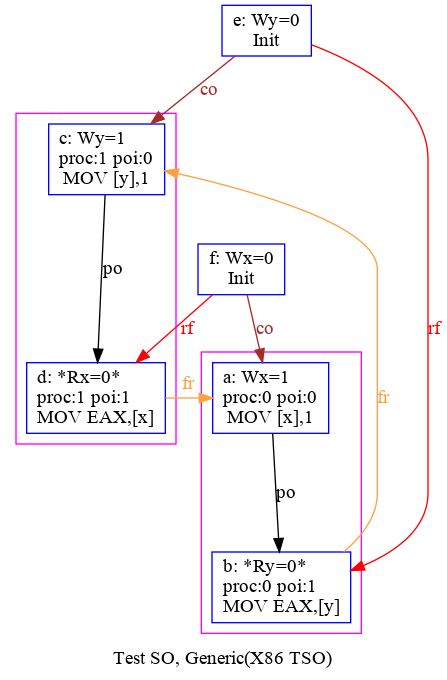
\includegraphics[width=0.4\textwidth]{img/my/simple_wmm_x86.png}
\begin{figure}
\centering
\begin{subfigure}[t]{.28\textwidth}
  \centering
  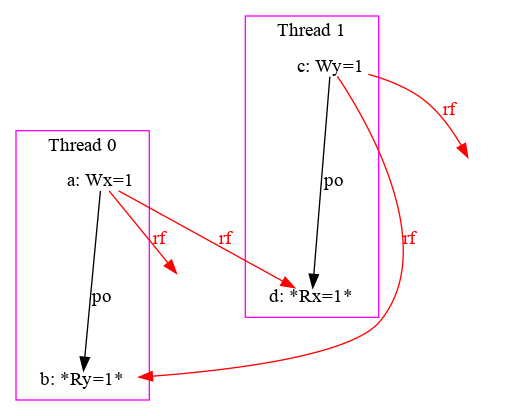
\includegraphics[width=1.2\linewidth]{img/my/sb-example/SB-dot.png}
  \caption{Final state: \texttt{(0:EAX=1~/\textbackslash~1:EAX=1)}}
  \label{simple_wmm_x86_pic:sub1}
\end{subfigure}
\hfill
\begin{subfigure}[t]{.23\textwidth}
  \centering
  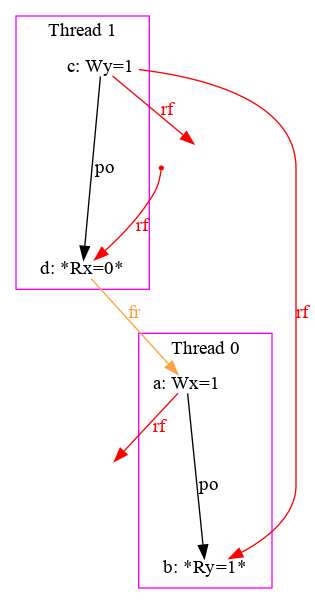
\includegraphics[width=.9\linewidth]{img/my/sb-example/SB-dot-2.png}
  \caption{Final state: \texttt{(0:EAX=1~/\textbackslash~1:EAX=0)}}
  \label{simple_wmm_x86_pic:sub2}
\end{subfigure}
\hfill
\begin{subfigure}[t]{.23\textwidth}
  \centering
  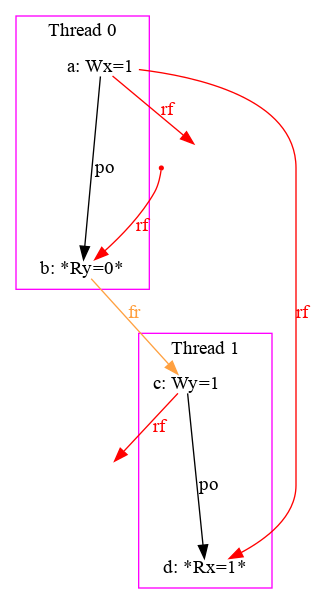
\includegraphics[width=.9\linewidth]{img/my/sb-example/SB-dot-3.png}
  \caption{Final state: \texttt{(0:EAX=1~/\textbackslash~1:EAX=1)}}
  \label{simple_wmm_x86_pic:sub3}
\end{subfigure}
\hfill
\begin{subfigure}[t]{.23\textwidth}
  \centering
  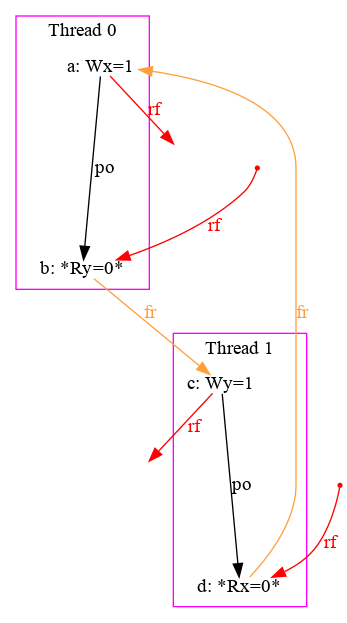
\includegraphics[width=.9\linewidth]{img/my/sb-example/SB-dot-4.png}
  \caption{Final state: \texttt{(0:EAX=0~/\textbackslash~1:EAX=0)}}
  \label{simple_wmm_x86_pic:sub4}
\end{subfigure}
\hfill
\caption{Candidate executions for the litmus test Example~\ref{simple_wmm_x86}}
\label{simple_wmm_x86_pic}
\end{figure}


\subsection{Weak Memory Models}
\label{ch:wmm:wmm}

\section{The \cat language}

Weak memory models can be described in the \cat language~\cite{alglave2016syntax}. It is the domain specific language for describing consistency properties of concurrent programs. The \cat language combines the expressive power of a functional language (it is inspired by OCaml and adopts its types, first-class functions, pattern matching and other features) with types, expressions and assertions specific for operating with relations and sets of executions.
% succinctly by constraining an abstraction of parallel program executions into a candidate execution and possibly extending this candidate execution with additional constraints on the execution environment.

%represents the functional language extended by the theory of  allows to axiomatically define derived relations, architecture-specific fences, and constraints over relations.

The definition of new relations  derived relations can be produced using the following operations over relations~\cite{alglave2016syntax}: % 3.1.6 Relations between events

\begin{itemize}
	\item \textit{the union} of two relations \texttt{r1} and \texttt{r2} is \texttt{r1\,|\,r2}
	\item \textit{the intersection} of two relations \texttt{r1} and \texttt{r2} is \texttt{r1\,\&\,r2}
	\item \textit{the difference} of two relations \texttt{r1} and \texttt{r2} is $\mathtt{r1\,\backslash\,r2}$
	\item \textit{the sequence}\footnote{The sequence of two relations \texttt{r1} and \texttt{r2} is defined as the set of pairs \texttt{(x,y)} such that there exists an intervening \texttt{z}, such that $\mathtt{(x,z)} \in \mathtt{r1}$ and $\mathtt{(z,y)} \in \mathtt{r2}$}
	of two relations \texttt{r1} and \texttt{r2} is \texttt{r1;r2}
\end{itemize}




%// exmaple with reordering
%// ex. with 
%// Rev-29 Example 7-6. Stores Are Transitively Visible. %see http://www.cl.cam.ac.uk/~pes20/weakmemory/x86tso-paper.pdf

%There is a barrier instruction \texttt{mfence} that may be used for flushing the buffers into the main memory.

briefly some hw memory models: X86-TSO, Alpha, POWER, ;

language memory models: Java, C++;

library-level kernel memory model, ref to github with tests

%Relationship between different models \url{http://wiki.expertiza.ncsu.edu/index.php/CSC/ECE_506_Spring_2013/10c_ks}


\section{Some examples of WMM}

//axioms of TSO wmm

// example of sets: rf, co, ... for the code snipped used before

